\usepackage{xeCJK}
\usepackage{array}
\usepackage{fancyhdr}
\usepackage{longtable}
\usepackage{graphics}
\usepackage{color}
\usepackage[left=2.5cm,right=2.5cm,top=2.5cm,bottom=2.5cm]{geometry}
\usepackage{hyperref}
\usepackage{listings}
\usepackage{xcolor}
\usepackage{titlesec}
\usepackage{float}
%\usepackage{CJKnumb}
\setCJKmainfont{WenQuanYi Micro Hei}
\setmainfont{Times New Roman}
\setsansfont{Arial}

\lstset{numbers=left, 
numberstyle=\tiny,
keywordstyle=\color{red!80}, 
frame=single,
basicstyle=\sffamily,
breaklines,
backgroundcolor=\color{red!60!green!60!blue!60},
commentstyle=\color{red!40!green!40!blue!40}, 
rulesepcolor=\color{red!20!green!20!blue!20}%,
%morekeywords={self,return}
}
%\titleformat{\chapter}{\Large}{第\,\CJKnumber{\thechapter}\,章}{1em}{}
%\titleformat{\section}{\large}{第\,\CJKnumber{\thesection}\,节}{1em}{}

\titleformat{\chapter}{\Large}{\underline{第\,\thechapter\,章}}{0em}{\underline}


\titleformat{\section}{\large}{第\,\thesection\,节}{0em}{}

\begin{document}%主体文档开始
\fancyhf{}
\pagestyle{fancy}
\fancyfoot[L]{}
\fancyfoot[C]{Tkinter8.5参考}
\fancyfoot[R]{\thepage}
\renewcommand{\footrulewidth}{0.4pt}

\frontmatter
\title{\huge \textbf{\textsf{Tkinter 8.5 参考:一个Python的图形界面}}}
\author{原文作者:\textsf{Joh W.Shipman}\\译者:\href{mailto:william0victor@gmail.com}{\textsf{William}}}
\date{原文发布时间:\textsf{2013-06-24 12:46}}
\linespread{1}
\maketitle


%摘要部分
\section*{摘要}

\subsection*{
本参考介绍了用Python编程语言中的Tkinter套件来创建用户图形界面。本参考涵盖了ttk主题控件。
}
\subsection*{
本参考现可\href{http://www.nmt.edu/tcc/help/pubs/tkinter/}{在线浏览\footnotemark[1]}同时另有\href{http://www.nmt.edu/tcc/help/pubs/tkinter/tkinter.pdf}{PDF文档\footnotemark[2]}。如有意见请发邮件到\href{mailto:tcc-doc@nmt.edu}{\textsf{tcc-doc@nmt.edu}}。
}
\subsection*{
如对翻译有任何意见请发邮件至\href{mailto:william0victor@gmail.com}{\textsf{william0victor@gmail.com}}
}
\footnotetext[1]{\href{http://www.nmt.edu/tcc/help/pubs/tkinter/}{http://www.nmt.edu/tcc/help/pubs/tkinter/}}
\footnotetext[2]{\href{http://www.nmt.edu/tcc/help/pubs/tkinter/tkinter.pdf}{http://www.nmt.edu/tcc/help/pubs/tkinter/tkinter.pdf}}

\renewcommand\contentsname{\textbf{目录}} 
\tableofcontents
\mainmatter

%第一章
\chapter[Python的一个跨平台用户图形界面]{Python的一个跨平台用户图形界面}
\textit{Tkinter}是Python的一个GUI(graphical user interface)组件。本文档适用于运行在Linux操作系统的X Window系统中的Python2.7和Tkinter8.5。你的版本或稍有差异。
\\
相关参考:
\begin{itemize}

\item Fredrik Lundh, who wrote \textit{Tkinter}, has two versions of his \textit{An Introduction to Tkinter}: \href{http://www.pythonware.com/library/tkinter/introduction/}{a more complete 1999 version}\footnotemark[3] and \href{http://effbot.org/tkinterbook/}{a 2005 version}\footnotemark[4] that presents a few newer features. 

\item \textit{\href{http://www.nmt.edu/tcc/help/pubs/python/}{Python 2.7 quick reference}}\footnotemark[5]{: general information about the Python language}

\item For an example of a sizeable working application (around 1000 lines of code), see huey: \href{http://www.nmt.edu/tcc/help/lang/python/examples/huey/}{\textit{A color and font selection tool}}\footnotemark[6]. 

\end{itemize}

我们将从\textit{Tkinter}可见的部分开始:创建控件并布局在屏幕上。稍后我们将探讨如何将应用程序前端的面板关联到后端逻辑。

\footnotetext[3]{\href{http://www.pythonware.com/library/tkinter/introduction/}{http://www.pythonware.com/library/tkinter/introduction/}}
\footnotetext[4] {\href{http://effbot.org/tkinterbook/}{http://effbot.org/tkinterbook/ }}
\footnotetext[5] {\href{http://www.nmt.edu/tcc/help/pubs/python/ }{http://www.nmt.edu/tcc/help/pubs/python/ }}
\footnotetext[6] {\href{http://www.nmt.edu/tcc/help/lang/python/examples/huey/}{http://www.nmt.edu/tcc/help/lang/python/examples/huey/}}
%第二章
\thispagestyle{fancy}
\chapter[一个小程序]{一个小程序}
下面是一个只含有一个推出按钮的\textit{Tkinter}小程序
\begin{lstlisting}[language=python]
#!/usr/bin/env python					1
import Tkinter as tk 					2
class Application(tk.Frame): 				3
	def __init__(self, master=None):	
		tk.Frame.__init__(self, master) 	4
		self.grid() 				5
		self.createWidgets()
	def createWidgets(self):
		self.quitButton = tk.Button(self, text='Quit',
			command=self.quit) 		6
		self.quitButton.grid() 			7
app = Application() 					8
app.master.title('Sample application') 			9
app.mainloop()						10
\end{lstlisting}
\begin{enumerate}
\item %1
假如你的系统中已正确安装Python,该行将会使脚本自动执行。
\item %2
该行将\textit{Tkinter}模块导入到程序的命名空间,但重命名为tk。
\item %3
你的程序的类必须从\textit{Tkinter}的Frame类继承。
\item %4
调用父类Frame的构造函数。
\item %5
必须让程序真正显示在屏幕上。
\item %6
创建一个按钮,标记为“Quit”。
\item %7
将按钮放入程序中
\item %8
通过实例化Application类启动主程序
\item %9
这个方法将窗口的title设为''Sample application''。
\item %10
启动程序的主程,等待鼠标和键盘事件。

\end{enumerate}

%第三章
\chapter[解释]{解释}
在我们继续下面的内容前,让我们来解释一些常用的名词。
\subsection*{window}
\indent
在不同的语境中这个词有不同的意思,但通常它是指你电脑显示屏中的某个矩形区域。
\subsection*{top-level window}
\indent
一个独立存在于你屏幕中的窗口,它将为你的系统桌面管理器装饰框架和控制器。你可以在桌面上四处移动它。通常,你也可以调整它的尺寸除非程序禁止了。
\subsection*{widget}
\indent
这个词通常指组成程序用户图形界面的组件。例如:按钮、单选框、文本域、框架以及文本标签。
\subsection*{frame}
\indent
在\textit{Tkinter}中,Frame控件是组成复杂布局的基本单元。它指一个能够包含其它控件的矩形区域。
\subsection*{child,parent}
\indent
当任意一个控件被创建时,父级-子级关系就已经建立。例如,当你将一个文本标签放入一个框架中,框架就是文本标签的父级。

%第四章
\chapter[布局管理]{布局管理}
接下来我们将讲讲控件,组成程序图形界面的“积木块”。怎样布置控件到窗口中?
尽管在\textit{Tkinter}中有三种不同“图形管理器”,但是笔者特别愿意用.grid()图形管理器来布局。这个管理将所有的窗口或框架当做一个表---有行和列的网格。
\begin{itemize}
\item
单元格是一行和一列的交叉区域。
\item
每列最宽的单元格的宽度是该列的列宽。
\item
每行最高的单元格的高度是该行的行高。
\item
控件不可能完全充满单元格的所有空间,你可以对单元格进行指定。你既可以不调整控件外的多余控件,也可以伸展水平方位或垂直方位来使控件填满单元格。
\item
你可以将多个单元格合并生成一个大单元格。
\end{itemize}
当你创建了一个控件,除非你在图形管理器中注册了它否则它将不显示。因此,构造和放置控件的两个步骤进行如下:
\begin{lstlisting}[language=python]
self.thing = tk.Constructor(parent, ...)
self.thing.grid(...)
\end{lstlisting}
\textit{Constructor}是如按钮、框架等控件的类,\textit{Parent}是将被构造的子类控件的父类控件。所有的控件都有.grid()方法,你可以使用它来告诉图形管理器怎么放置控件。

%第4.1节
\section[.grid()方法]{.grid()方法}
将一个控件\textit{W}显示到程序窗口中:
\begin{lstlisting}[language=python]
w.grid(option=value, ...)
\end{lstlisting}
该方法在图形管理器中注册了一个控件\textit{w}---如果不这么做,控件将只存在内部不会显示出来。见表一“.grid()图形管理器参数”:
\begin{longtable}{|l|p{0.85\textwidth}|}

\hline
\textsf
column &
控件放置的列数,从0开始计算。默认值是0。\\ \hline
columnspan & 
通常一个控件只占据网格中的一个单元格。然而,你可以选取行中的多个单元格,并在columnspan选项中设置单元格的数量来整合他们到一个大单元格。例如,\textit{w}.grid(row=0,column=2,columnspan=3),例中将会把\textit{w}控件放置在一个横跨0行2,3,4列的一个单元格中。\\ \hline
in\_ &
注册\textit{w}作为某个控件如\textit{w$_2$}的子类,用法in\_=\textit{w$_2$}。当\textit{w}被创建时,新的\textit{w$_2$}控件必须作为\textit{parent}控件的子类来使用。\\ \hline
ipadx &
内部x padding。这个维度是增加控件内部左边和右边。\\ \hline
ipady &
内部y padding。这个维度是增加控件内部顶部和底部。\\ \hline
padx &
外部x padding。这个维度是增加控件外部左边和右边。\\ \hline
pady &
外部y padding。这个维度是增加控件上部和下部。\\ \hline
row &
你想把控件插入的行数,从0计数。默认是下一个更高的未被占用的行。\\ \hline
rowspan &
通常一个控件只占据网格的一个单元格。你可以选取列内的多个单元格,然后,给选中的单元格设置rowspan选项。本选项和columnspan选项结合使用来抓取一块单元格。例子,\textit{w}.grid(row=3,column=2,rowspan=4,columnspan=5)例中将\textit{w}微件放入一个由3-6列2-6行组成的区域中。\\ \hline
sticky &
本项决定怎样分配单元格中的微件所占空间之外的空间。见下。\\ \hline
\end{longtable}

\begin{itemize}
\item 如果未设置sticky属性,默认会将微件在单元格中居中放置。

\item 你可以使用sticky=NE(右上),SE(右下),SW(左下),或者NW(左上)来布局微件到单元格的四角。

\item 你可以使用sticky=N(中上),E(中右),S(中下),或者W(中左)来布局微件到一边的相对中间。

\item 使用sticky=N+S垂直扩展微件但让它水平居中。

\item 使用sticky=E+W水平扩展微件但让它垂直居中。

\item 使用sticky=N+E+S+W在水平和垂直方位来扩展微件填充单元格。

\item 其它的组合也可使用。例如,sticky=N+S+W将垂直扩展微件并放置微件在相对东(左)边。
\end{itemize}

%第4.2章
\section{其它grid管理方法}
这些grid相关的方法在所有控件上都有定义:
\subsection*{\textsf{\textit{w}.grid\_bbox ( column=None, row=None, col2=None, row2=None )}}
\par{返回一个四元组描述微件w中一些或所有grid系统的边界框。前两个数字返回左上角区域的x和y坐标,后两个数字是宽和高。}
\par{如果你传递行和列变量,返回的限定框描述所在行和列的单元格的区域。如果你也传递了col2和row2参数,返回的限定框描述包含从行column到col2,列row到row2的区域。}
\par{例如,w.grid\_bbox(0,0,1,1)返回四个单元格的限定框,不是一个。}

\subsection*{\textsf{\textit{w}.grid\_forget()}}
\par{本方法使微件w从屏幕上消失。它还存在,只是不可见。你可以使用.grid()使它再次显示,但是它将不会记住它的grid选项。}

\subsection*{\textsf{\textit{w}.grid\_info()}}
\par{返回一个键为w微件选项名字的字典,以及这些选项相应的值。}

\subsection*{\textsf{\textit{w}.grid\_location (x,y)}}
\par{赋予关联的包含的微件一个坐标,本方法返回一个数组(col,row)描述w微件的网格系统的单元格包含的屏幕坐标。}

\subsection*{\textsf{\textit{w}.grid\_propagate()}}
\par{通常,所有微件传送他们的尺寸,意味着他们调节来适应内容。然而,有时你想约束一个微件到确定的尺寸,忽略它内容的尺寸,这样做,调用w.grid\_propagate(0)限制w微件的尺寸。}

\subsection*{\textsf{\textit{w}.grid\_remove()}}
\par{本方法类似.grid\_forget() ,但是它的grid选项会记住 ,所以如果你再.grid()它 ,它将会使用相同的grid配置选项。}

\subsection*{\textsf{\textit{w}.grid\_size()}}
\par{分别在w微件grid系统中返回一个包含行数和列数的二元组。}

\subsection*{\textsf{\textit{w}.grid\_slaves ( row=None, column=None )}}
\par{返回由微件w管理的微件的目录。如果没有提供参数,你将会获得所有被管理的微件的目录。使用row=参数只选择一列微件,或者使用column=参数只选择一行的微件。}

%第4.3章
\section{配置列和行的尺寸}
除非你采取确切的措施,网格列内的微件宽将会等于它的最大宽度,并且网格行内的控件高将会是最高的单元格的高。控件里的sticky属性只控制控件被放置的地方如果所在单元格未被完全填充满。

\subsection*{\textsf{\textit{w}.columnconfigure ( N, option=value,...)}}
\par{w微件的网格层中, 配置column N以便所给选项有所给的值。对于选项,请看下表。}

\subsection*{\textsf{\textit{w}.rowconfigure ( N, option=value, … )}}
\par{w微件的网格层中,配置row N以便所给的选项有所给的值。对于选项,请看下表。}

以下是用来配置column和row尺寸的选项。\\
\begin{tabular}{|l|p{0.85\textwidth}|}
\hline
minsize&
以像素为最小单位,列和行的最小尺寸。如果列内或行内没有内容,它将不会显示即使你使用了这一选项\\ \hline
pad&
若干像素将会被加入所给的列或行,及以上的列或行中最大的单元格。\\ \hline
weight&
为了使一列或一行可伸展,当重新分配额外的空间时,使用此选项并提供一个值,赋予该列或行相对权重。例如,如果一个微件w包含一个网格层,这些行将会分配3/4的额外空间到第一列及1/4到第二列:
\begin{lstlisting}[language=python]
w.columnconfigure(0, weight=3)
w.columnconfigure(1, weight=1)
\end{lstlisting}
如果没有使用此项,列或行将不会伸展。\\ \hline
\end{tabular}

%第4.4章
\section{让根窗口可重组}
你想让用户能调整你的整个程序窗口大小,并将空出的控件分配给内部的控件吗?只需普通的几个操作就能实现。

这需要用到行和列尺寸管理的方法,在第4.3小节已经提到,“配置列和行大小”(p.7),来使你的\textit{Application}控件的网格可伸缩。然而,那仅仅是不够的。

思考下第二章讨论的小程序,“一个小程序”(p.2),这个程序只包含一个退出按钮。如果你运行此程序,并调整窗口大小,按钮会保持同样的尺寸,并居中于窗口。

以下是小程序内.\_\_createWidgets()方法的替代版本。在这个版本中,退出按钮总是填满可用空间。
\begin{lstlisting}[language=python]
def createWidgets(self):
	top=self.winfo_toplevel()					1
	top.rowconfigure(0,weight=1)	   				2
	top.columnconfigure(0,weight=1)					3
	self.rowconfigure(0,weight=1)					4
	self.columnconfigure(0,weight=1)				5
	self.quit=Button (self, text=”Quit”, command=self.quit )
	self.quit.grid( row=0, column=0, sticky=N+S+E+W)		6
\end{lstlisting}
\begin{enumerate}
\item “top level window''是屏幕上最顶层的窗口。但是,这个窗口不是\textit{Application}的窗口——它是\textit{Application}实例的父级。要获取顶层窗口,在程序中的任何控件上调用.winfo\_toplevel()方法。参看章节,“通用控件方法”(p.97)。
\item 本行代码使top level window的0列网格可伸展。 
\item 本行代码使顶层窗口的0列网格可伸展。
\item 使0行的\textit{Application}控件的网格可伸展。
\item 使0列的\textit{Application}控件的网格可伸展
\item 参数sticky=tk.N+tk.S+tk.E+tk.W使按钮展开填满它所占的单元格
\end{enumerate}
还必须作出一个变化。在构造函数中,如下显示的改变第二行:
\begin{lstlisting}[language=python]
def __init__(self,master=None):
	Frame.__init__(self,master)
	self.grid(sticky=tk.N+tk.S+tk.E+tk.W)
	self.createWidgets()
\end{lstlisting}
sticky=tk.N+tk.S+tk.E+tk.W参数对self.grid()是必要的,因此\textit{Application}控件将会展开填充它所在top-level window网格的单元格。


%第五章
\chapter{标准属性}


在我们看控件之前,让我们来看看他们的一些共同指定的属性---如大小,颜色以及字体。
\begin{itemize}
\item
每个控件都有一些属性选项来影响它的显示和行为,如颜色,大小,文本标签等。
\item
当调用控件构造器时,你可以使用如text='PANIC'或者height=20等关键字参数。
\item
当你创建了一个控件后,后面你可以使用控件的.config()方法来改变参数。你也可以使用控件的.cget()方法来获取当前参数的设置。了解更多类似方法请看第26章“通用控件方法”(P.97)
\end{itemize}

%第5.1节
\section{尺寸}

控件的长,宽及其它的尺寸可以用许多不同的单位。
\begin{itemize}
\item
如果你想设置一个整数尺寸,它将默认以像素为单位
\item
你可以在设定尺寸时在数字后加入如下字符来指定单位:
\end{itemize}
\hspace{4em}
表3.尺寸单位

\hspace{2em}
\begin{tabular}{r|l}
\hline
c & Centimeters \\ \hline
i & Inches \\ \hline
m & Millimeters \\ \hline
p & Printer's points (about 1/72'') \\ \hline
\end{tabular}

\section{坐标系}
%As in most contemporary display systems, the origin of each coordinate system is at its upper left corner,
%with the x coordinate increasing toward the right, and the y coordinate increasing toward the bottom:
当前的大多数显示系统中,坐标系是在左上角,x轴向右走,y轴向下走:

\begin{figure}[H]
\hspace{1em}
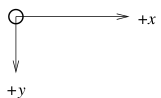
\includegraphics[width=5.680cm,height=3.457cm]{5.2.png}
\end{figure}

%The base unit is the pixel, with the top left pixel having coordinates (0,0). Coordinates that you specify
%as integers are always expressed in pixels, but any coordinate may be specified as a dimensioned
%quantity; see Section 5.1, “Dimensions” (p. 9).
最基本的单位是像素,最左上的像素的坐标为(0,0)。你所指定的整数坐标通常默认以像素为单位,但是坐标都可能指定数值;请见第5.1节“尺寸”(P.9)

%第5.3节
\section{颜色}
\textit{Tkinter}中一般有两种方法来指定颜色
\begin{itemize}
\item
你可以通过16进制字符设置红、绿、蓝颜色的比例来设置颜色:
\\
\begin{tabular}{|l|l|}
\hline
\textsf{\#rgb} & Four bits per color \\ \hline
\textsf{\#rrggbb} & Eight bits per color \\ \hline
\textsf{\#rrrgggbbb} & Twelve bits per color \\ \hline
\end{tabular}
\\
%For example, '#fff' is white, '#000000' is black, '#000fff000' is pure green, and '#00ffff'
%is pure cyan (green plus blue).
例如,“\textsf{\#fff}”是白色,“\textsf{\#000000}”是黑色,“\textsf{\#000fff000}”是纯绿色,“\textsf{\#00ffff}”是青色(绿色加蓝色)
\item
另外你也可以使用内置的标准颜色名。\textsf{white}白色,\textsf{black}黑色,\textsf{red}红色,\textsf{green}绿色,\textsf{blue}蓝色,\textsf{cyan}青色,\textsf{yellow}黄色,\textsf{magenta}品红都能用。其它颜色名也许也能用,要看本地安装环境。

\end{itemize}

\end{document}%主体文档结束